\documentclass[11pt,a4paper]{article}
\usepackage[utf8]{inputenc}
\usepackage[T1]{fontenc}
\usepackage{lmodern}
\usepackage{microtype}
\usepackage[a4paper,margin=1in]{geometry}
\usepackage{amsmath,amssymb,amsthm,mathtools}
\usepackage{booktabs,array,enumitem,tabularx}
\usepackage{graphicx}
\usepackage{xcolor}
\definecolor{accent}{HTML}{1F3A5F}
\usepackage[colorlinks=true,linkcolor=accent,citecolor=accent,urlcolor=accent]{hyperref}
\usepackage{sectsty}
\usepackage{fancyhdr}
\usepackage{setspace}
\setstretch{1.2}
\sectionfont{\color{accent}}\subsectionfont{\color{accent}}
\pagestyle{fancy}\fancyhf{}
\rhead{\small\itshape Constrained Arbitrage under India's Limits}\lhead{\small BS Project: Theoretical Framework}
\cfoot{\thepage}\renewcommand{\headrulewidth}{0.4pt}

\newcommand{\E}{\mathbb{E}}
\DeclarePairedDelimiter{\abs}{\lvert}{\rvert}
\theoremstyle{plain}
\newtheorem{proposition}{Proposition}
\newtheorem{lemma}{Lemma}
\newtheorem{corollary}{Corollary}
\theoremstyle{definition}
\newtheorem{assumption}{Assumption}
\theoremstyle{remark}
\newtheorem*{remark}{Remark}
\newtheorem*{test}{Empirical content}

\title{\vspace{-1.2cm}\color{accent}\bfseries Constrained Arbitrage under India's Limits:\\ A Model of the Basis, the F\&O Ban and Short-Sale Constraints\\[0.25cm]
\large\mdseries\color{black} Theoretical framework for the BS Project}
\author{Prince Kumar (23B3032), BS Economics, IIT Bombay\\ \small Guide: Prof.\ Aditi Chaubal \quad\textbar\quad EC~495 / EC~497}
\date{October 2026}

\begin{document}
\maketitle
\thispagestyle{empty}

\begin{abstract}
\noindent This note sets out one model that covers the limits to arbitrage the project studies in Indian equities:
trading costs, the cost of shorting, arbitrage capital, arbitrage risk, position limits and the F\&O ban. Each limit is a
parameter of the same model, so every empirical hypothesis is derived from one framework. The core is a
mean--variance arbitrage sector that trades the futures--cash basis against outside traders in both markets. Three
features matter for the Indian setting. (i) The F\&O ban is modelled as it actually operates: a
\emph{reduce-only} rule for every participant, not a freeze on the arbitrageur alone. (ii) Arbitrage inventory is a state
variable, so the no-trade region moves with existing positions. (iii) Demand that is blocked from the futures market
can spill into the cash market. The main prediction is that the ban turns two-sided arbitrage into
\emph{one-sided} arbitrage: futures that are too cheap are still corrected (by unwinding existing cash-and-carry
positions), while futures that are too rich are not. The ban's effect on the \emph{level} of the basis is
\emph{ambiguous}, and the model states the observable conditions that sign it. It also implies that the MWPL
denominator is not a valid excluded instrument for ban status, because the same variable moves the probability of a
future ban. All closed forms are checked numerically (Appendix~\ref{app:num}). The note ends with a map from
propositions to hypotheses, each with the result that would contradict it.
\end{abstract}

\tableofcontents
\newpage

%=====================================================================
\section{Purpose}
The aim is to fix a theoretical framework before the empirical work, so that the hypotheses are derived rather than
fitted. The model builds on the limits-to-arbitrage literature (Shleifer and Vishny, 1997; Gromb and Vayanos, 2010) and
on the econometrics of no-arbitrage bands (Dwyer, Locke and Yu, 1996; Tse, 2001; Ters and Urban, 2020). Three design
rules guide it:
\begin{enumerate}[leftmargin=1.6em,itemsep=1pt]
\item \textbf{Institutions as they are.} The ban, the short-selling framework, settlement prices and costs are modelled
from the primary sources (SEBI circular 2025/79; NSE Clearing circular 119/2025 and its FAQ of October 2025).
\item \textbf{Predictions that can fail.} Wherever the sign of an effect depends on the environment, the model says on
what, and the empirical work tests that condition rather than a one-sided sign.
\item \textbf{Daily horizon.} The data are daily, so the relevant arbitrageur carries positions overnight
(arbitrage mutual funds, proprietary desks), not a one-second market maker.
\end{enumerate}

%=====================================================================
\section{Environment}\label{sec:env}
%=====================================================================
\subsection{Prices and the basis}
A stock with spot price $S_t$ has a single-stock future maturing at $T$. With benchmark rate $r_b$ (e.g.\ MIBOR) and
known dividends, the cost-of-carry value is $F^*_t=(S_t-\mathrm{PV}_t(D))\,e^{r_b(T-t)}$. The \emph{basis} (mispricing)
is
\begin{equation}
m_t \;=\; \ln F_t-\ln F^*_t ,
\end{equation}
measured in basis points of the spot price. Write $s$ and $f$ for the deviations of spot and futures prices from the
fundamental value, so $m=f-s$ to first order.

\subsection{Outside traders and market clearing}
Outside (non-arbitrage) traders in each market have linear demand. In the cash market net demand is $D_S-\psi_S s$, in
the futures market net long demand is $D_F-\psi_F f$; $\psi_S,\psi_F>0$ measure liquidity (the depth of the outside
side of each market) and $D_S, D_F$ are demand shifters. An arbitrage sector holds $a$ units of the cash-and-carry
trade: long $a$ shares and short $a$ futures ($a<0$ is reverse arbitrage). Both markets are in zero net supply after
removing the fundamental holdings, so
\begin{align}
D_S-\psi_S s + a &= 0, & D_F-\psi_F f - a &= 0 .
\end{align}
Subtracting, the basis satisfies
\begin{equation}\label{eq:clear}
m=\frac{u-a}{\Phi},\qquad \frac1\Phi\equiv\frac1{\psi_F}+\frac1{\psi_S},\qquad u\equiv \Phi\Big(\frac{D_F}{\psi_F}-\frac{D_S}{\psi_S}\Big).
\end{equation}
$u$ is the \emph{relative demand pressure} toward futures: positive when outside traders want long exposure in futures
more than in cash (e.g.\ leveraged speculative longs), negative when they want short exposure in futures (hedgers,
informed pessimists who can short only through futures). Without arbitrage the basis is $u/\Phi$; arbitrage lowers it by
$a/\Phi$ (buying cash raises $s$, selling futures lowers $f$).

\subsection{The arbitrage sector}
\begin{assumption}[Arbitrage]\label{as:arb}
The arbitrage sector is competitive and chooses $a$ to maximise
\begin{equation}\label{eq:obj}
\Pi(a)= a\,m-\tfrac{\gamma}{2}a^2 - c_+\,a^+ - c_-\,a^-,\qquad \gamma\equiv\alpha\sigma^2>0,
\end{equation}
where $a^\pm=\max(\pm a,0)$, $\alpha$ is risk aversion per unit of capital (inversely related to arbitrage capital),
$\sigma^2$ the basis risk borne until convergence (margin calls, early unwinds), $c_+$ the cost of a cash-and-carry
position and $c_-$ the cost of a reverse position.
\end{assumption}
Holding a unit of cash-and-carry to expiry earns $m$ (the basis converges to zero), less costs. Decomposing,
\begin{equation}\label{eq:costs}
c_+=\tau_+ + (r_A-r_b)(T-t),\qquad c_-=\tau_- + \big(\ell_s+r_b-r_L\big)(T-t),
\end{equation}
with $\tau_\pm$ the round-trip transaction costs of each trade (STT, stamp duty, exchange fees, brokerage, impact),
$r_A$ the required return of cash-and-carry capital, $\ell_s$ the stock-lending fee and $r_L$ the rebate on short
proceeds. Section~\ref{sec:map} maps each Indian limit to these parameters.

\subsection{Indian limits as parameters}
\begin{center}
\small
\begin{tabularx}{\textwidth}{>{\raggedright\arraybackslash}p{3.4cm}>{\raggedright\arraybackslash}X>{\raggedright\arraybackslash}p{3.0cm}}
\toprule
Limit & Indian institution (dated shocks) & Parameter \\
\midrule
Trading costs & STT on futures (sell side): 0.01\% from 1 Jun 2013; 0.0125\% from 1 Apr 2023; 0.02\% from 1 Oct 2024; 0.05\% from 1 Apr 2026. Cash delivery STT 0.1\% each side; 0.1\% on physically settled derivatives & $\tau_+,\tau_-$ \\
Short-sale cost & Naked shorting barred; only F\&O-segment securities are eligible for short selling and SLB; SLB thin; the overnight short is the future & $c_-$ via $\ell_s$; $c_-=\infty$ for cash-only stocks \\
Arbitrage capital & Arbitrage-fund AUM (tax-advantaged since the 1 Apr 2023 debt-fund tax change); funding rates; peak-margin phase-in (Dec 2020--Sep 2021) & $\alpha$ (so $\gamma$), $r_A$ \\
Arbitrage risk & Basis volatility, idiosyncratic volatility & $\sigma^2$ (so $\gamma$) \\
Position limits & Entity limits (10/20/30\% of MWPL from 1 Oct 2025); MWPL; the F\&O ban (95\% entry, 80\% exit) & caps on $a$; reduce-only rule (Sec.~\ref{sec:ban}) \\
Market depth & Liquidity of outside traders in each market & $\psi_S,\psi_F$ (so $\Phi$) \\
\bottomrule
\end{tabularx}
\end{center}

%=====================================================================
\section{The no-arbitrage band}\label{sec:band}
%=====================================================================
\begin{proposition}[Asymmetric band and passthrough]\label{prop:band}
Under Assumption~\ref{as:arb} and \eqref{eq:clear}, the equilibrium is unique:
\begin{equation}\label{eq:band}
m(u)=\begin{cases}
\dfrac{\gamma u + c_+}{\gamma\Phi+1}, & u>\Phi c_+,\\[2mm]
\dfrac{u}{\Phi}, & -\Phi c_-\le u\le \Phi c_+,\\[2mm]
\dfrac{\gamma u - c_-}{\gamma\Phi+1}, & u<-\Phi c_- ,
\end{cases}
\qquad
a(u)=\begin{cases}\dfrac{u-\Phi c_+}{\gamma\Phi+1}, & u>\Phi c_+,\\[1mm] 0, & \text{inside},\\[1mm] \dfrac{u+\Phi c_-}{\gamma\Phi+1}, & u<-\Phi c_-.\end{cases}
\end{equation}
The basis is left alone inside the band $[-c_-,\,c_+]$; outside it, arbitrage absorbs a share of each demand shock, so
the passthrough falls from $1/\Phi$ to $\gamma/(\gamma\Phi+1)$.
\end{proposition}
\begin{proof}
$\Pi$ is strictly concave with kinks at $0$. The best response is $a=(m-c_+)/\gamma$ if $m>c_+$, $a=(m+c_-)/\gamma$ if
$m<-c_-$, and $a=0$ otherwise. The map $a\mapsto \mathrm{BR}((u-a)/\Phi)-a$ is strictly decreasing, so the fixed point is
unique. Substituting $m=(u-a)/\Phi$ into the interior best responses gives \eqref{eq:band}; e.g.\ for the upper branch
$m\Phi=u-(m-c_+)/\gamma$, i.e.\ $m=(\gamma u+c_+)/(\gamma\Phi+1)$, which equals $c_+$ at $u=\Phi c_+$ (continuity).
\end{proof}

\begin{proposition}[Comparative statics]\label{prop:cs}
\begin{enumerate}[label=(\roman*),leftmargin=1.8em,itemsep=1pt]
\item \emph{Costs set the edges.} The band edges are $c_+$ and $-c_-$; they do not depend on capital or risk. A change in
transaction costs $\Delta\tau_\pm$ (e.g.\ an STT change) shifts the corresponding edge one-for-one.
\item \emph{Capital and risk set the passthrough.} Outside the band, $\partial m/\partial u=\gamma/(\gamma\Phi+1)$ rises with
$\gamma=\alpha\sigma^2$: scarcer capital or riskier convergence lets the basis travel further beyond the edge.
\item \emph{Maturity.} By \eqref{eq:costs} both edges are affine in remaining maturity $T-t$ and converge to the round-trip
costs $\tau_+$, $-\tau_-$ at expiry (for positions held to expiry).
\item \emph{Location.} The band is centred at $(c_+-c_-)/2$, below zero whenever shorting costs more than carrying
($c_->c_+$). Its \emph{upper} edge is itself negative when $(r_b-r_A)(T-t)>\tau_+$, i.e.\ when cash-and-carry capital
accepts a return sufficiently below the benchmark rate.
\end{enumerate}
\end{proposition}
\begin{proof}
(i)--(iii) follow from \eqref{eq:band} and \eqref{eq:costs}. (iv): the centre is $(c_+-c_-)/2$; the sign of $c_+$
follows from \eqref{eq:costs}.
\end{proof}

\begin{remark}
Part (iv) matters because the Indian evidence shows a band centred below zero: Shankar, Sankar and Kiran Kumar (2015)
estimate mean thresholds of $-39$ and $-10$ bp for 102 NSE stock futures (5-minute data, 2007--09), and the median basis
is negative in Aggarwal (2015) and Nandan et al.\ (2014). The model reproduces this if reverse arbitrage is costly and
cash-and-carry capital accepts a below-benchmark return. One candidate is the tax treatment of arbitrage funds, which
are taxed as equity. If so, the inflows after the 1 April 2023 debt-fund tax change should have lowered $r_A$ and with it
the upper edge, which is a testable implication. It must be separated from the futures STT increase on the same date, which
raises $\tau_+$.
\end{remark}

%=====================================================================
\section{Inventory and the moving no-trade region}\label{sec:inv}
%=====================================================================
The ban acts on existing positions, so the model needs inventory. Time is discrete (days). The arbitrage sector enters
day $t$ with inventory $a_{t-1}\ge 0$ and pays proportional costs on changes: $c_+$ per unit added and $c_u$ per unit
unwound (selling cash, buying back futures). To keep the dynamic analysis transparent, reverse arbitrage is set aside
($a_t\ge 0$): the capacity of stock \emph{holders} to sell cash and buy futures when futures are cheap is part of the
cash-market depth $\psi_S$. Each day the sector chooses $a_t$ to maximise
\begin{equation}\label{eq:dynobj}
a_t m_t-\tfrac{\gamma}{2}a_t^2 - c_+(a_t-a_{t-1})^+ - c_u(a_{t-1}-a_t)^+ .
\end{equation}

\begin{proposition}[Inventory-dependent no-trade region]\label{prop:inv}
Given $a_{t-1}$, the sector trades only when the basis leaves
\begin{equation}
\big[\,\gamma a_{t-1}-c_u,\;\; \gamma a_{t-1}+c_+\,\big].
\end{equation}
In equilibrium, with $m^0_t\equiv(u_t-a_{t-1})/\Phi$:
\begin{enumerate}[label=(\alph*),leftmargin=1.8em,itemsep=1pt]
\item if $m^0_t>\gamma a_{t-1}+c_+$ the sector adds: $m_t=(\gamma u_t+c_+)/(\gamma\Phi+1)$;
\item if $m^0_t<\gamma a_{t-1}-c_u$ it unwinds: $a_t=\max\{0,(u_t+\Phi c_u)/(\gamma\Phi+1)\}$ and $m_t=(u_t-a_t)/\Phi$;
\item otherwise $a_t=a_{t-1}$ and $m_t=m^0_t$.
\end{enumerate}
\end{proposition}
\begin{proof}
\eqref{eq:dynobj} is strictly concave with kinks at $a_{t-1}$. The marginal value of the position is $m_t-\gamma a_t$, so
adding is optimal iff $m_t-\gamma a_{t-1}>c_+$ and unwinding iff $m_t-\gamma a_{t-1}<-c_u$; interior solutions are
$a_t=(m_t-c_+)/\gamma$ and $a_t=(m_t+c_u)/\gamma$. Uniqueness and the closed forms follow as in
Proposition~\ref{prop:band}, combining each branch with \eqref{eq:clear}.
\end{proof}

\begin{test}
Thresholds are not constants: they rise with arbitrage inventory. A large existing cash-and-carry book (proxied by
open interest built while the basis was rich) raises both the level at which new arbitrage starts and the level at which
unwinding starts. Threshold models should allow thresholds to depend on lagged OI.
\end{test}

%=====================================================================
\section{The F\&O ban as a reduce-only rule}\label{sec:ban}
%=====================================================================
\subsection{The rule}
Once market-wide open interest in a stock's derivatives exceeds 95\% of its MWPL at the end of a day, the stock enters the
ban from the next day. Every entity may then only trade to reduce its position (from 1 October 2025, its end-of-day
futures-equivalent delta); a change of sign counts as a violation. Normal trading resumes when open interest falls to
80\% of MWPL (NSE Clearing circular 119/2025). The rule covers all expiries and options; rolling a position into the next
expiry is not permitted. It binds outside traders as much as arbitrageurs.

\begin{assumption}[Ban]\label{as:ban}
During a ban:
\begin{enumerate}[label=(B\arabic*),leftmargin=2.2em,itemsep=1pt]
\item \emph{Reduce-only arbitrage:} $0\le a_t\le a_{t-1}$.
\item \emph{Blocked new exposure:} outside traders' demand shocks have two parts, $\Delta u_t=\varepsilon^n_t+\varepsilon^c_t$
in normal times. Closing demand $\varepsilon^c_t$ (long liquidation, short covering) can still be executed and enters as
usual. Demand for \emph{new} futures exposure $\varepsilon^n_t$ cannot; a share $\chi\in[0,1]$ of it moves to the cash
market and the rest is withdrawn. In the units of \eqref{eq:clear} the ban maps $\varepsilon^n_t$ into
$-\lambda\varepsilon^n_t$, with $\lambda\equiv\chi\,\psi_F/\psi_S\ge 0$.
\end{enumerate}
\end{assumption}
(B2) follows from \eqref{eq:clear}: new long demand $\Delta D_F=\varepsilon$ raises $u$ by $\Phi\varepsilon/\psi_F$ if it
enters futures, but lowers $u$ by $\Phi\chi\varepsilon/\psi_S$ if a share $\chi$ of it buys cash instead. A leveraged
retail trader who cannot buy the future and buys the stock on margin is the leading case.

\begin{lemma}\label{lem:weak}
For the same $u_t$ and $a_{t-1}$, the basis in a ban is at least as high as in normal times.
\end{lemma}
\begin{proof}
(B1) removes only the option to add, which is used only when it lowers $m$ (branch (a) of Proposition~\ref{prop:inv});
branches (b)--(c) are unchanged.
\end{proof}

\begin{proposition}[One-sided correction]\label{prop:onesided}
Let a ban start with inventory $a_{t-1}>0$.
\begin{enumerate}[label=(\roman*),leftmargin=1.8em,itemsep=1pt]
\item \emph{No ceiling.} For $u_t\ge a_{t-1}(1+\gamma\Phi)-\Phi c_u$ the basis is $m_t=(u_t-a_{t-1})/\Phi$: every increase
in pressure passes through fully ($\partial m/\partial u=1/\Phi$ instead of $\gamma/(\gamma\Phi+1)$ beyond the normal
upper edge). Rich futures are not corrected.
\item \emph{A floor while inventory lasts.} For lower $u_t$ the sector unwinds and $m_t=\gamma a_t-c_u$, so cheap futures
are still corrected, at a level that \emph{rises} with the remaining inventory.
\item \emph{The floor wears out.} Once $a_t=0$ the floor disappears and $m_t=u_t/\Phi$. Because positions cannot be rolled,
an expiry inside a ban removes the expiring part of the inventory for the rest of the ban.
\end{enumerate}
\end{proposition}
\begin{proof}
Apply Proposition~\ref{prop:inv} with branch (a) deleted by (B1). Branch (c) holds while
$m^0_t\ge\gamma a_{t-1}-c_u$, i.e.\ $u_t\ge a_{t-1}(1+\gamma\Phi)-\Phi c_u$, giving (i). In branch (b), $a_t=(m_t+c_u)/\gamma$
when interior, so $m_t=\gamma a_t-c_u$, giving (ii). If $(u_t+\Phi c_u)\le 0$ then $a_t=0$ and $m_t=u_t/\Phi$, giving
(iii). Expiry: delivered positions close and cannot be re-opened in the next expiry under the ban.
\end{proof}

\begin{proposition}[Sign reversal of new-exposure demand]\label{prop:flip}
In normal times a shock to demand for new futures exposure moves the basis in its own direction:
$\partial m_t/\partial\varepsilon^n_t=1/\Phi$ inside the no-trade region and $\gamma/(\gamma\Phi+1)$ beyond its upper edge.
In a ban the same shock moves it the other way: $\partial m_t/\partial\varepsilon^n_t=-\lambda/\Phi$ inside the no-trade
region and $-\lambda\gamma/(\gamma\Phi+1)$ on the unwinding floor. The reversal is strict iff $\chi>0$.
\end{proposition}
\begin{proof}
Chain rule on Propositions~\ref{prop:inv}--\ref{prop:onesided}, with $\partial u/\partial\varepsilon^n=1$ in normal times and
$-\lambda$ in a ban by (B2).
\end{proof}

\begin{proposition}[The level effect is ambiguous]\label{prop:level}
Fix $a_{t-1}$, the pre-shock pressure $u^0$ and closing demand $\varepsilon^c$, and compare the same new-exposure shock
$\varepsilon^n\ge0$ with and without a ban: $m^N=m(u^0+\varepsilon^c+\varepsilon^n)$ and
$m^B=m^{ban}(u^0+\varepsilon^c-\lambda\varepsilon^n)$. Then:
\begin{enumerate}[label=(\roman*),leftmargin=1.8em,itemsep=1pt]
\item $m^B-m^N$ is non-increasing in $\varepsilon^n$;
\item at $\varepsilon^n=0$, $m^B-m^N\ge0$, strictly if closing pressure would have triggered new arbitrage in normal times;
\item $m^B-m^N<0$ for $\varepsilon^n$ large enough.
\end{enumerate}
The ban \emph{raises} the basis when pressure comes mainly from closing trades (e.g.\ short covering) and \emph{lowers} it
when new speculative demand keeps arriving; the observable sign condition is the composition of order flow during the ban.
\end{proposition}
\begin{proof}
$m^N$ is non-decreasing in $\varepsilon^n$; $m^B$ is non-increasing in $\varepsilon^n$ because $u^B$ falls in $\varepsilon^n$
and $m^{ban}$ is non-decreasing in $u$. Hence (i). (ii) is Lemma~\ref{lem:weak}. (iii): $m^N$ rises without bound (slope
at least $\gamma/(\gamma\Phi+1)>0$) while $m^B$ is non-increasing.
\end{proof}

\begin{proposition}[Trading and measurement in a ban]\label{prop:trade}
\begin{enumerate}[label=(\roman*),leftmargin=1.8em,itemsep=1pt]
\item If the reduce-only rule binds contract by contract, every futures trade in a ban closes a long and a short, so
$\Delta OI_t=-V_t$ (volume) outside expiry days. Trades that offset across instruments (e.g.\ delta-reducing option trades
allowed from 1 October 2025) break the identity; the gap measures such offsetting.
\item Trading requires that some long and some short both want to reduce at the same price, so futures volume falls
and quoted spreads widen relative to normal days.
\item On days without trades in the last half hour, NSE sets the futures settlement price at a theoretical cost-of-carry
value. The settlement-price basis is then zero by construction (up to differences between NSE's rate and $r_b$).
\end{enumerate}
\end{proposition}
\begin{proof}
(i) A buyer may only reduce a short and a seller only reduce a long, so each trade lowers OI by its size. (ii) follows from
the restriction of the trading set. (iii) is the NSE settlement rule.
\end{proof}

\begin{remark}
Part (iii) is a trap for the empirics. Bans thin out trading, so a naive basis built from settlement prices would show the
basis ``closing'' during bans for purely mechanical reasons. The data work must use trade-based prices and flag
theoretical settlements.
\end{remark}

%=====================================================================
\section{Anticipation and hysteresis}\label{sec:antic}
%=====================================================================
\begin{assumption}[Exit in a ban is costlier]\label{as:exit}
If a ban occurs before a position is closed, unwinding costs $c_u+\ell$ with $\ell>0$, because the counterparties are only
traders who also want to reduce (Prop.~\ref{prop:trade}(ii)). The probability that a position opened when utilisation is
$\omega=OI/MWPL$ meets a ban before it is closed is $\pi(\omega)$, continuous and increasing.
\end{assumption}

\begin{proposition}[Anticipation]\label{prop:antic}
Outside a ban the effective cost of opening cash-and-carry is $c_+ + \pi(\omega)\ell$. The upper edge of the no-trade
region rises smoothly as utilisation approaches 95\%, and new arbitrage slows before any ban. The jump at $\omega=0.95$
consists only of the reduce-only effects of Section~\ref{sec:ban}; anticipation is continuous through the threshold.
\end{proposition}
\begin{proof}
The expected cost of a unit opened at $\omega$ is $c_++\pi(\omega)\ell$ (exit at a later date is costlier with probability
$\pi$); substitute for $c_+$ in Proposition~\ref{prop:inv}. Continuity of $\pi$ gives continuity at $0.95$.
\end{proof}

\begin{remark}[What the density of utilisation should look like]
Arbitrageurs hold back as $\omega$ rises, which thins the density just below 95\%; speculators who expect a ban may rush to
open positions first, which does the opposite. The model therefore does not sign a McCrary test; the test tells us which
force dominates.
\end{remark}

\begin{corollary}[Hysteresis]\label{cor:hyst}
For $\omega\in[0.80,0.95)$ a stock may be in a ban (it crossed 95\% earlier) or not. At the same $\omega$ the first is
governed by Section~\ref{sec:ban}, the second by Proposition~\ref{prop:antic}. Their difference is the effect of the
reduce-only state relative to the anticipation state, which is the effect the 95/80 rule creates.
\end{corollary}

%=====================================================================
\section{What the model implies for identification}\label{sec:id}
%=====================================================================
\begin{proposition}[MWPL is not a clean instrument for ban status]\label{prop:id}
The basis depends on the MWPL through three channels: the ban state $B_t=B(\omega_t,B_{t-1})$, the anticipation term
$\pi(\omega_t)$, and entity limits proportional to the MWPL when they bind. A change in the MWPL therefore moves the
basis even in periods with no ban, so it violates the exclusion restriction for an instrument of $B_t$. Denominator
variation identifies the \emph{total} effect of the position-limit regime (ban plus anticipation plus caps), not the effect
of the ban alone.
\end{proposition}
\begin{proof}
$\omega=OI/MWPL$ enters $\pi(\omega)$ (Prop.~\ref{prop:antic}) independently of $B$.
\end{proof}

What each design identifies under the model:
\begin{enumerate}[leftmargin=1.6em,itemsep=1pt]
\item \emph{RD at 95\%}: the local jump in the reduce-only effects, provided utilisation cannot be placed precisely on one side.
\item \emph{Hysteresis comparison} (Cor.~\ref{cor:hyst}): the reduce-only state against the anticipation state at equal $\omega$;
selection on past paths must be controlled (lagged utilisation, lagged basis).
\item \emph{Ban-entry event study with near-miss controls}: Props.~\ref{prop:onesided}--\ref{prop:trade} dynamically, against
stocks with similar paths that stayed below 95\%.
\item \emph{1 October 2025 reform and quarterly MWPL recalculations}: reduced-form effects of predicted changes in utilisation
(new formula; FutEq numerator) on the basis. These are total-regime effects (Prop.~\ref{prop:id}).
\end{enumerate}

%=====================================================================
\section{Short-sale constraints beyond the basis}\label{sec:short}
%=====================================================================
\subsection{Earnings news in a ban}
\begin{proposition}[Bad news is incorporated more slowly in a ban]\label{prop:news}
Let an announcement reveal news $\pm\delta$, and let trading on the day impound a share $k$ of it. For bad news, a share
$\rho$ of informed selling capacity runs through short futures, the only overnight short in an F\&O stock. In a ban that
capacity is unavailable, so the share impounded falls to $k(1-\rho)$ and the post-announcement drift after bad news rises
from $(1-k)\delta$ to $(1-k+k\rho)\delta$. Good news is unaffected because optimists can buy cash.
\end{proposition}
\begin{proof}
Immediate from the definitions; the asymmetry comes from the fact that the cash market allows buying but not overnight
selling by non-holders.
\end{proof}
\begin{remark}
Outside a ban the same mechanism predicts that informed pessimists push the futures price \emph{below} carry before bad
news, since their short futures cannot be met by reverse arbitrage. A recent working paper (Saurav, Srivastava and
Agarwalla, 2026) reports a negative basis before earnings announcements in Indian stock futures. The model adds that this pre-announcement signal should \emph{vanish} for stocks in a ban, while drift after
bad news should grow.
\end{remark}

\subsection{Cash-only stocks and F\&O inclusion}
Stocks outside the F\&O segment have no single-stock futures and are not eligible for short selling or SLB under SEBI's
framework, so $c_-$ is effectively infinite for overnight positions. A Miller (1977) mechanism then applies.

\begin{proposition}[Overpricing without a short channel]\label{prop:miller}
A continuum of investors has valuations $v_i\sim U[v-\delta,v+\delta]$ and demands $k(v_i-p)$ if long; shorting costs $c_s$
per unit, so investors with $v_i<p-c_s$ short $k(v_i-p+c_s)$. Supply is $Q>0$.
\begin{enumerate}[label=(\roman*),leftmargin=1.8em,itemsep=1pt]
\item The price $p(c_s)$ is non-decreasing in $c_s$.
\item With free shorting $p=v-Q/k$. With no shorting and $\delta\ge Q/k$, $p=v+\delta-2\sqrt{\delta Q/k}$, so the
overpricing is $\big(\sqrt{\delta}-\sqrt{Q/k}\big)^2$, increasing in dispersion $\delta$.
\end{enumerate}
\end{proposition}
\begin{proof}
(i) Aggregate demand falls in $p$ and rises in $c_s$ (short positions shrink), so the market-clearing price rises in $c_s$.
(ii) Free shorting: $\int k(v_i-p)\,di=k(v-p)=Q$. No shorting: $\frac{k}{2\delta}\int_p^{v+\delta}(x-p)\,dx=\frac{k(v+\delta-p)^2}{4\delta}=Q$,
valid when $p\ge v-\delta$, i.e.\ $\delta\ge Q/k$. Subtract; the derivative in $\delta$ is $1-\sqrt{Q/(k\delta)}>0$.
\end{proof}
\begin{test}
F\&O inclusion lowers $c_s$ (futures, options, short-selling and SLB eligibility arrive together). It should lower
prices of high-dispersion stocks at inclusion and reduce their subsequent underperformance; exclusion should do the
reverse. Diamond and Verrecchia (1987) imply that, even without a level bias, short constraints slow the incorporation of
bad news, which points in the same direction as Proposition~\ref{prop:news}.
\end{test}

%=====================================================================
\section{Heterogeneous arbitrageurs and the estimation lens}\label{sec:het}
%=====================================================================
With a single cost $c_+$ the band has sharp edges and, under impulse-style correction, the outer regimes would almost never
be observed. Let costs differ across arbitrageurs, $c\sim G$ on $[\underline c,\bar c]$, each with the objective
\eqref{eq:obj}. Aggregate arbitrage is $a(m)=\int (m-c)^+\,dG(c)/\gamma$, which is continuous and convex in $m$ above
$\underline c$, so the strength of correction rises smoothly with the size of the deviation. In discrete time, with capital
moving to opportunities only gradually, the basis follows an error-correction process whose speed of adjustment is a
smooth, increasing function of $|m_{t-1}-\text{centre}|$. This is the exponential or logistic smooth-transition model (Tse, 2001).
It is also well approximated by a three-regime threshold model whose thresholds are quantiles of $G$ (Dwyer, Locke and Yu,
1996; Ters and Urban, 2020). Proposition~\ref{prop:inv} adds that the thresholds move with inventory, and
Proposition~\ref{prop:onesided} that in a ban the upper regime's adjustment speed falls toward zero while the lower regime's
remains. A band-of-inaction (impulse-control) derivation gives the same reading for a single arbitrageur: the threshold is
the point at which correcting the deviation becomes worth its cost.

%=====================================================================
\section{Calibration and horizon}\label{sec:cal}
%=====================================================================
For an overnight carrier, the round-trip cost of a cash-and-carry trade includes STT on the cash purchase and sale
(0.1\% each), STT on the futures sale (0.01--0.05\% depending on the period) or 0.1\% on physical delivery, stamp duty,
exchange and clearing fees, brokerage and impact. That is tens of basis points, far wider than the bands of a few
basis points estimated from one-second data (Aggarwal, 2015), which describe intraday market makers. Arbitrage funds that roll rather than deliver spread these costs over several expiries, which
lowers the effective $\tau_+$ per month. The empirical work will compute a bottom-up cost band for each period; the simulations here
use round illustrative numbers ($c_+=15$, $c_u=10$, $c_-=60$ bp) and are not estimates.

%=====================================================================
\section{From propositions to hypotheses}\label{sec:map}
%=====================================================================
\begin{center}
\small
\begin{tabularx}{\textwidth}{>{\raggedright\arraybackslash}p{0.8cm}>{\raggedright\arraybackslash}p{2.3cm}>{\raggedright\arraybackslash}X>{\raggedright\arraybackslash}X}
\toprule
H & Source & Prediction & What would contradict it \\
\midrule
H1 & Props.~\ref{prop:band}--\ref{prop:inv} & Mispricing size and persistence rise with ex-ante frictions & No relation between friction index and band/persistence \\
H2 & Props.~\ref{prop:news}, \ref{prop:miller} & Drift after bad news larger without a short channel (cash-only stocks; ban days); good news unaffected & Symmetric drift response, or larger effect for good news \\
H3 & Prop.~\ref{prop:cs}(i),(iii) & Edges move one-for-one with cost changes (STT 2023, 2024, 2026); edges shrink toward expiry; estimated band close to cost band & Band unrelated to dated cost changes \\
H4 & Prop.~\ref{prop:cs}(ii),(iv) & Scarcer capital widens excursions beyond the edges; tax-advantaged inflows lower the upper edge & Basis level unaffected by arbitrage-fund flows (after separating the 1 Apr 2023 STT change) \\
H5 & Prop.~\ref{prop:miller} & Overpricing-side anomalies stronger where shorting is costly; underpricing side unaffected & Symmetric effect on both legs \\
H6 & Prop.~\ref{prop:miller} & F\&O inclusion lowers overpricing, more for high-dispersion stocks; exclusion raises it & No change, or opposite sign \\
H7 & Prop.~\ref{prop:onesided} & In a ban, positive deviations stop reverting; negative ones still revert while inventory lasts, less after an expiry in the ban & Symmetric change, or no change \\
H8 & Props.~\ref{prop:flip}, \ref{prop:trade} & In a ban, futures volume falls, $\Delta OI\approx -V$, cash activity rises; response of the basis to new-demand shocks flips sign & Futures activity unchanged; no sign flip \\
H9 & Props.~\ref{prop:antic}, \ref{prop:id}, Cor.~\ref{cor:hyst} & Upper edge rises smoothly as utilisation nears 95\%; the 1 Oct 2025 package acts through predicted utilisation, with sign set per stock & Jump only at 95\% with no pre-trend; no effect of predicted utilisation \\
\bottomrule
\end{tabularx}
\end{center}
The level effect of the ban (Prop.~\ref{prop:level}) is deliberately \emph{not} a one-sided hypothesis: the test is whether
its sign follows the composition of order flow (closing versus new demand) as the model says.

%=====================================================================
\section{Limitations}
%=====================================================================
\begin{enumerate}[leftmargin=1.6em,itemsep=1pt]
\item Partial equilibrium with linear outside demand and a myopic, mean--variance arbitrage sector; dynamic hedging and
the option to unwind early (Brennan and Schwartz, 1990) enter only through the inventory structure.
\item The split of outside demand into closing and new-exposure parts (B2) is the modelling choice that drives
Props.~\ref{prop:flip}--\ref{prop:level}. Its empirical counterpart (order flow that opens versus closes positions) is only
partly observable from public data (changes in OI against volume).
\item Reverse arbitrage by stock holders is folded into cash-market depth, not modelled as a separate agent.
\item Anticipation rests on Assumption~\ref{as:exit} (costlier exit in a ban), which is itself testable (Prop.~\ref{prop:trade}(ii)).
\item Propositions~\ref{prop:news}--\ref{prop:miller} are deliberately simple; they fix directions, not magnitudes.
\end{enumerate}

\appendix
%=====================================================================
\section{Numerical verification and illustration}\label{app:num}
%=====================================================================
A Python script solves each equilibrium by brute force (bisection on the best-response fixed point) and compares it
with the closed forms. All checks pass: the static band (Prop.~\ref{prop:band}),
the inventory step in normal times and in a ban (Props.~\ref{prop:inv}--\ref{prop:onesided}), the floor
$\gamma a_t-c_u$ and the full passthrough above it, Lemma~\ref{lem:weak}, the monotonicity and sign change in
Proposition~\ref{prop:level}, and the Miller closed forms (Prop.~\ref{prop:miller}).

The simulation uses illustrative parameters ($\Phi=\gamma=1$; $c_+=15$, $c_u=10$ bp; demand pressure AR(1) with
persistence 0.9 around 25 bp; daily shock s.d.\ 6 bp for each component; $\lambda=0.5$). Each experiment runs the same
shocks with and without a 40-day ban.
\begin{itemize}[leftmargin=1.6em,itemsep=1pt]
\item \emph{Asymmetric reversion} (300 episodes): the slope of $\Delta m_t$ on $m_{t-1}$ above the 80th percentile weakens
from $-0.18$ (no ban) to $-0.13$ (ban); below the 20th percentile it strengthens from $-0.12$ to $-0.16$.
\item \emph{Level effect}: with no extra new-exposure demand during the ban the mean basis is $+4.9$ bp higher; with a
steady inflow of 1, 2 and 4 bp/day of new demand it is $-3.1$, $-10.8$ and $-26.0$ bp lower (Prop.~\ref{prop:level}).
\end{itemize}

\begin{figure}[h]
\centering
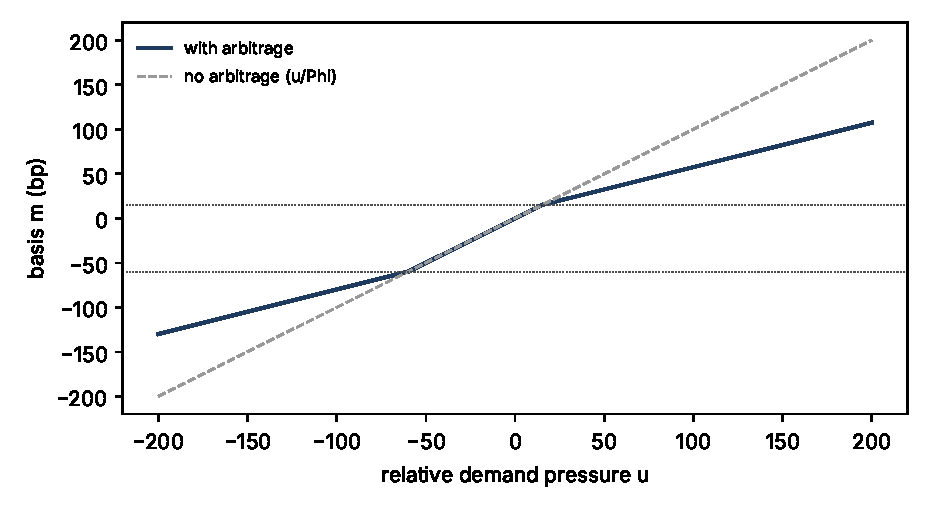
\includegraphics[width=0.78\textwidth]{figs/fig_band.pdf}
\caption{Static equilibrium (Prop.~\ref{prop:band}): the basis follows demand pressure one-for-one inside the band and is
compressed outside it. Dotted lines: edges $c_+$ and $-c_-$.}
\end{figure}
\begin{figure}[h]
\centering
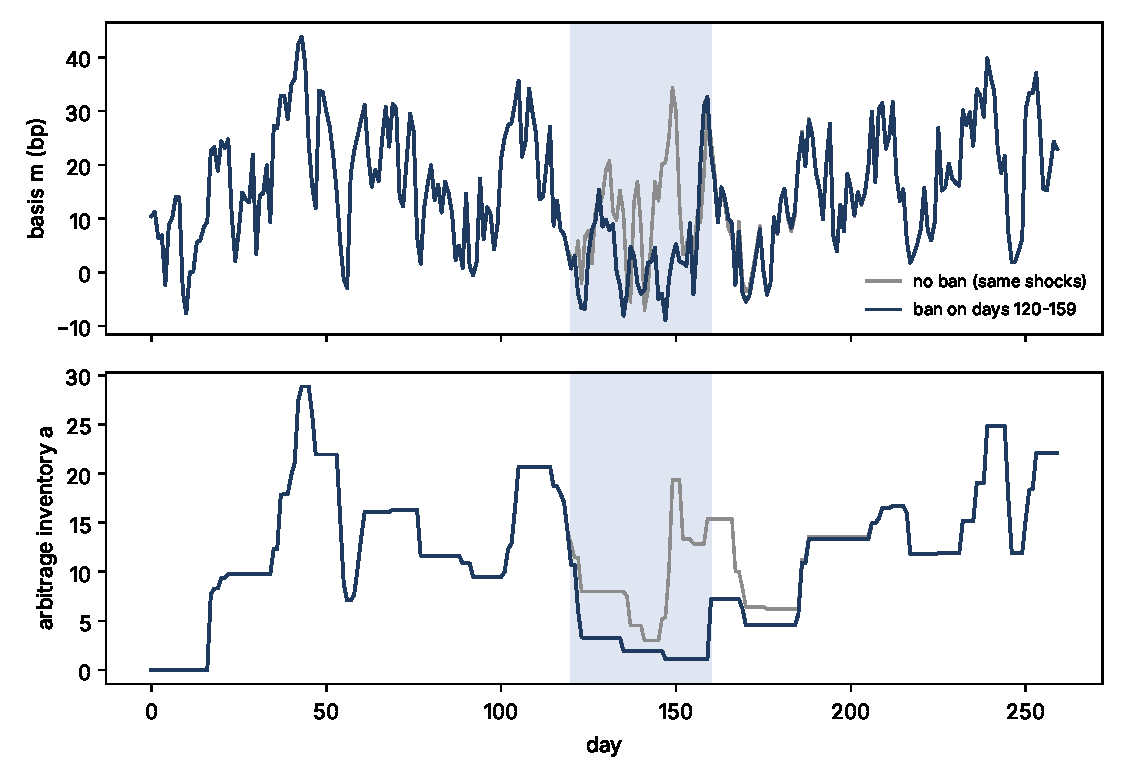
\includegraphics[width=0.85\textwidth]{figs/fig_path.pdf}
\caption{One simulated path, same shocks with and without a ban on days 120--159. In the ban, inventory can only fall and
upward pressure passes through fully.}
\end{figure}
\begin{figure}[h]
\centering
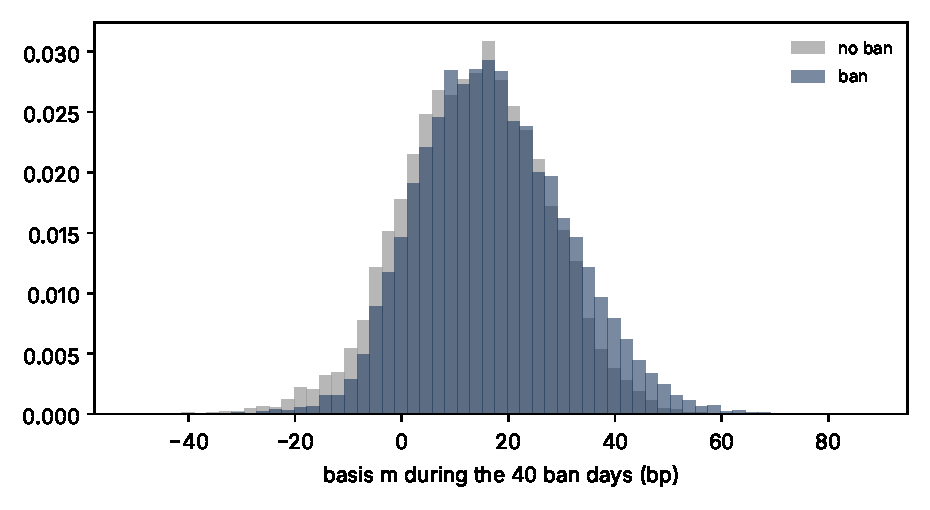
\includegraphics[width=0.78\textwidth]{figs/fig_hist.pdf}
\caption{Distribution of the basis over the 40 ban days, pooled across 300 paired simulations.}
\end{figure}

\clearpage
\section*{References}
\small
\begin{description}[leftmargin=1.2em,itemsep=0pt,font=\normalfont]
\item Aggarwal, N. (2015). Limits to arbitrage: The case of single stock futures and spot prices. IGIDR WP-2015-010.
\item Brennan, M. and E. Schwartz (1990). Arbitrage in stock index futures. \emph{Journal of Business} 63(1), S7--S31.
\item Diamond, D. and R. Verrecchia (1987). Constraints on short-selling and asset price adjustment to private information. \emph{Journal of Financial Economics} 18, 277--311.
\item Dwyer, G., P. Locke and W. Yu (1996). Index arbitrage and nonlinear dynamics between the S\&P 500 futures and cash. \emph{Review of Financial Studies} 9(1), 301--332.
\item Gromb, D. and D. Vayanos (2010). Limits of arbitrage. \emph{Annual Review of Financial Economics} 2, 251--275.
\item Miller, E. (1977). Risk, uncertainty, and divergence of opinion. \emph{Journal of Finance} 32(4), 1151--1168.
\item Nandan, T., P. Agrawal and S. Bhargava (2014). Mispricing in CNX Nifty futures: An empirical investigation. \emph{Asia-Pacific Journal of Management Research and Innovation} 10(4), 413--422.
\item NSE Clearing (2025). Circular 119/2025, 8 September 2025; FAQ on position limits, limit monitoring and securities in ban period, updated 13 October 2025.
\item Saurav, S., P. Srivastava and S. K. Agarwalla (2026). Decoupled: Disagreement, short-sale constraints, and law-of-one-price violations around earnings announcements. SSRN working paper.
\item SEBI (2025). Measures for enhancing trading convenience and strengthening risk monitoring in equity derivatives. Circular SEBI/HO/MRD/TPD-1/P/CIR/2025/79, 29 May 2025.
\item Shankar, R.L., G. Sankar and K. Kiran Kumar (2015). Mispricing in single stock futures: Empirical examination of Indian markets. NSE Working Paper WP/16/2015; \emph{Emerging Markets Finance and Trade} 55(7), 1619--1633 (2019).
\item Shleifer, A. and R. Vishny (1997). The limits of arbitrage. \emph{Journal of Finance} 52(1), 35--55.
\item Ters, K. and J. Urban (2020). Estimating unknown arbitrage costs: Evidence from a 3-regime threshold vector error correction model. \emph{Journal of Financial Markets} 47, 100503.
\item Tse, Y. (2001). Index arbitrage with heterogeneous investors: A smooth transition error-correction analysis. \emph{Journal of Banking \& Finance} 25(10), 1829--1855.
\end{description}
\end{document}
